\documentclass{ocbeameruni}


\setdefaultlanguage[babelshorthands=true]{german}


% Nur benötigt für die Beispiel-Listings!
\usepackage{listings}
\usetikzlibrary{arrows}
\lstloadlanguages{[LaTeX]TeX}
\lstset{%
  basicstyle=\small \ttfamily,
  breaklines=true,
}

\newcommand{\R}{\mathbb{R}}


\title{Organic Computing 2}
\subtitle{Lösungsvorschlag Blatt05}
\date{\today}
\author{Lukas Huhn \and Qiang Chang \and Victor Gerling}
\institute{%
  Universität Augsburg\\
  Institut für Informatik\\
  Lehrstuhl für Organic Computing
}


\begin{document}


\maketitle


\begin{frame}{Gliederung}
  \setbeamertemplate{section in toc}[sections numbered]
  \tableofcontents
\end{frame}

\section{Aufgabe 02}

\begin{frame}{Black-Box 1}
    \begin{center}
    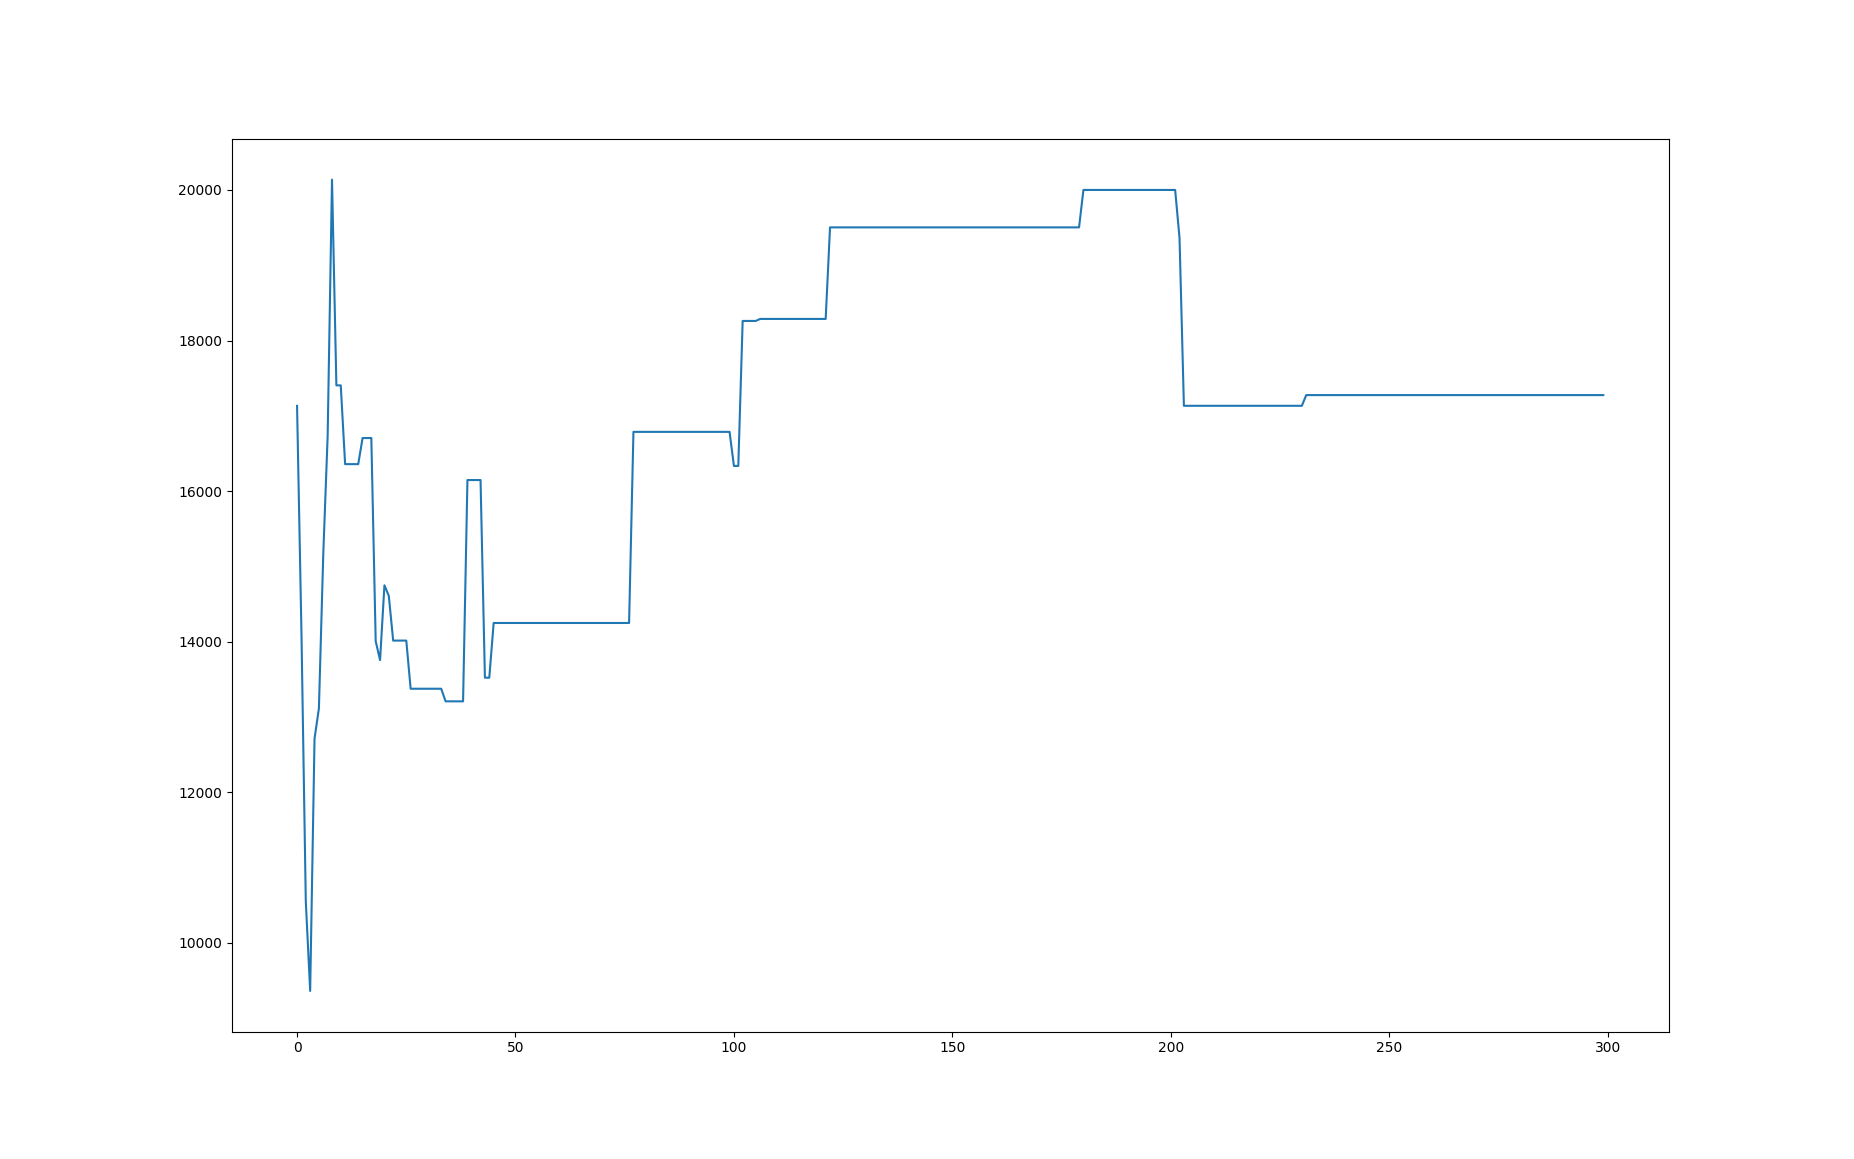
\includegraphics[scale=0.2]{plots/bb1.png}
    \end{center}
\end{frame}

\begin{frame}{Black-Box 2}
    \begin{center}
    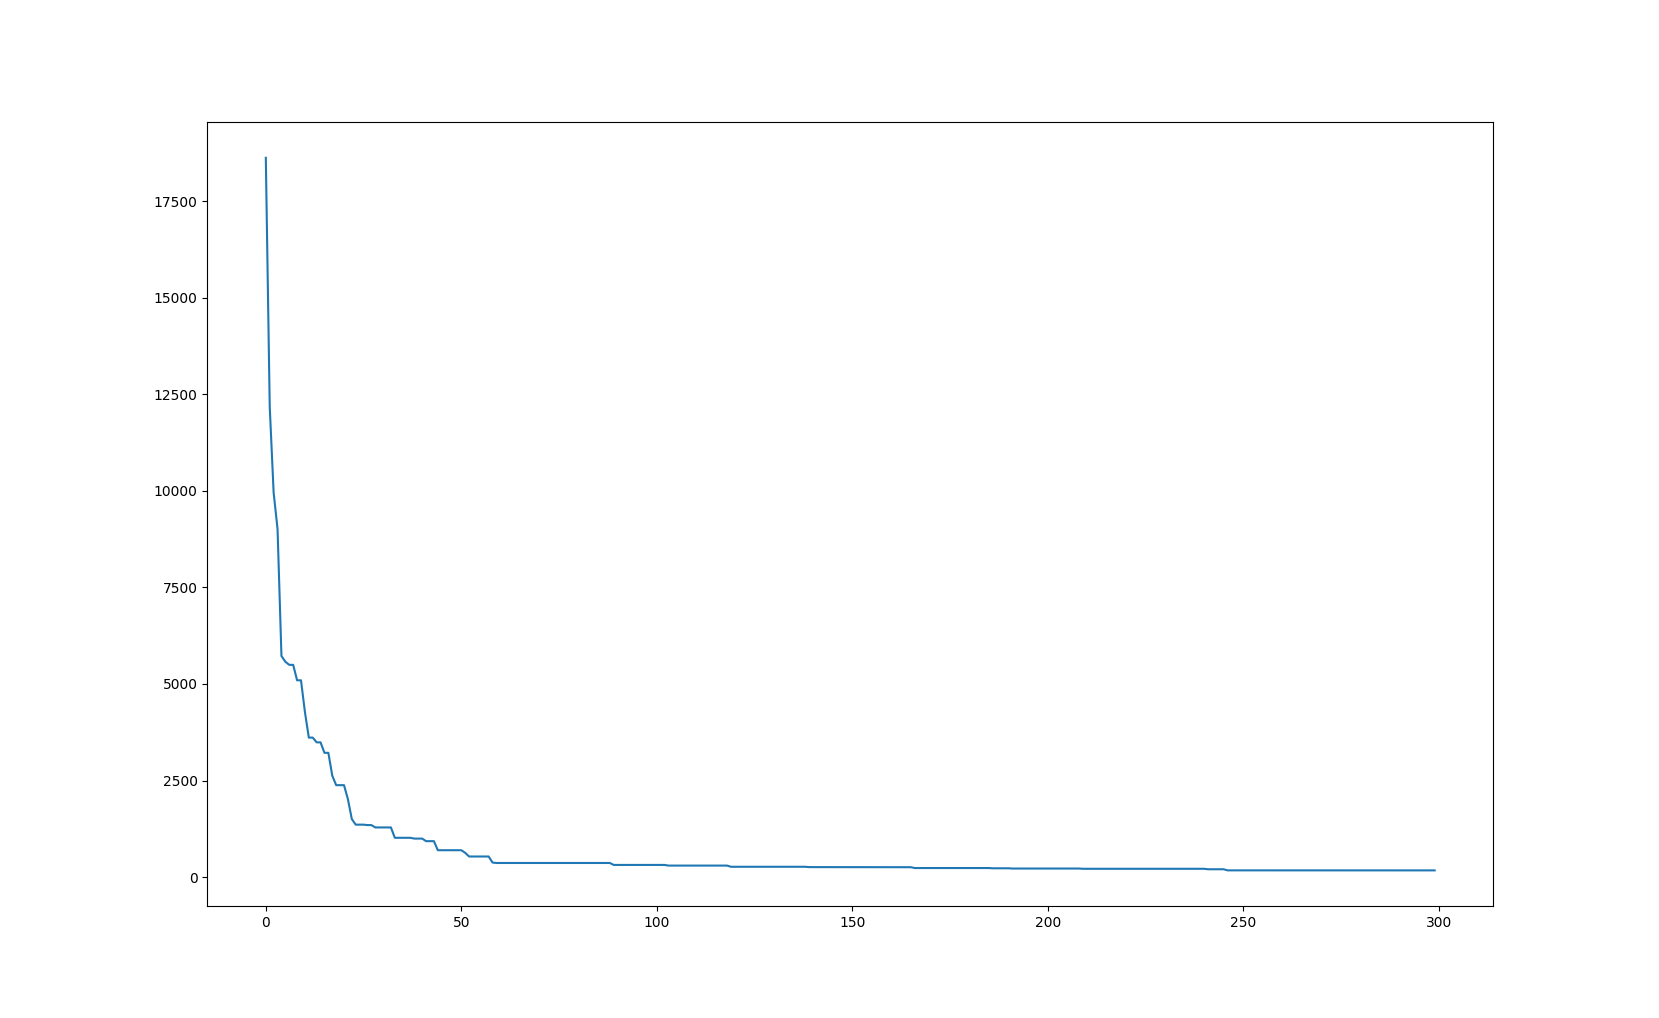
\includegraphics[scale=0.25]{plots/bb2.png}
    \end{center}
\end{frame}

\begin{frame}{Black-Box 3}
    \begin{center}
    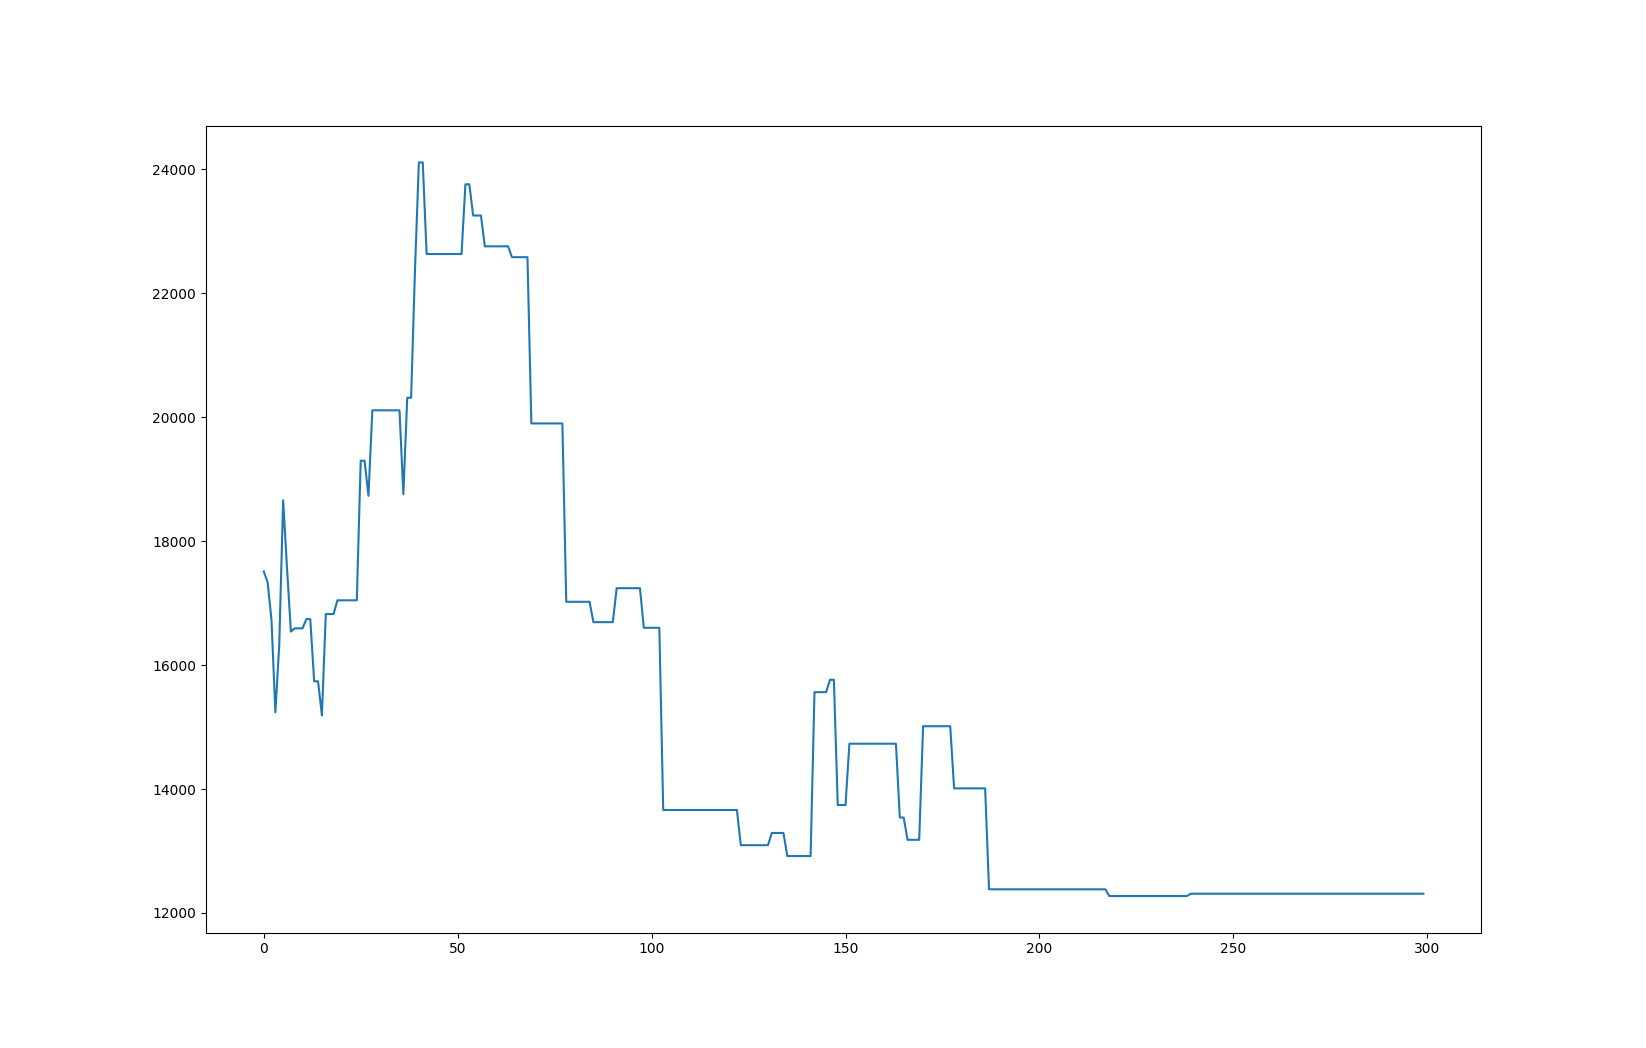
\includegraphics[scale=0.3]{plots/bb3.png}
    \end{center}
\end{frame}

\begin{frame}{Black-Box 4}
    \begin{center}
    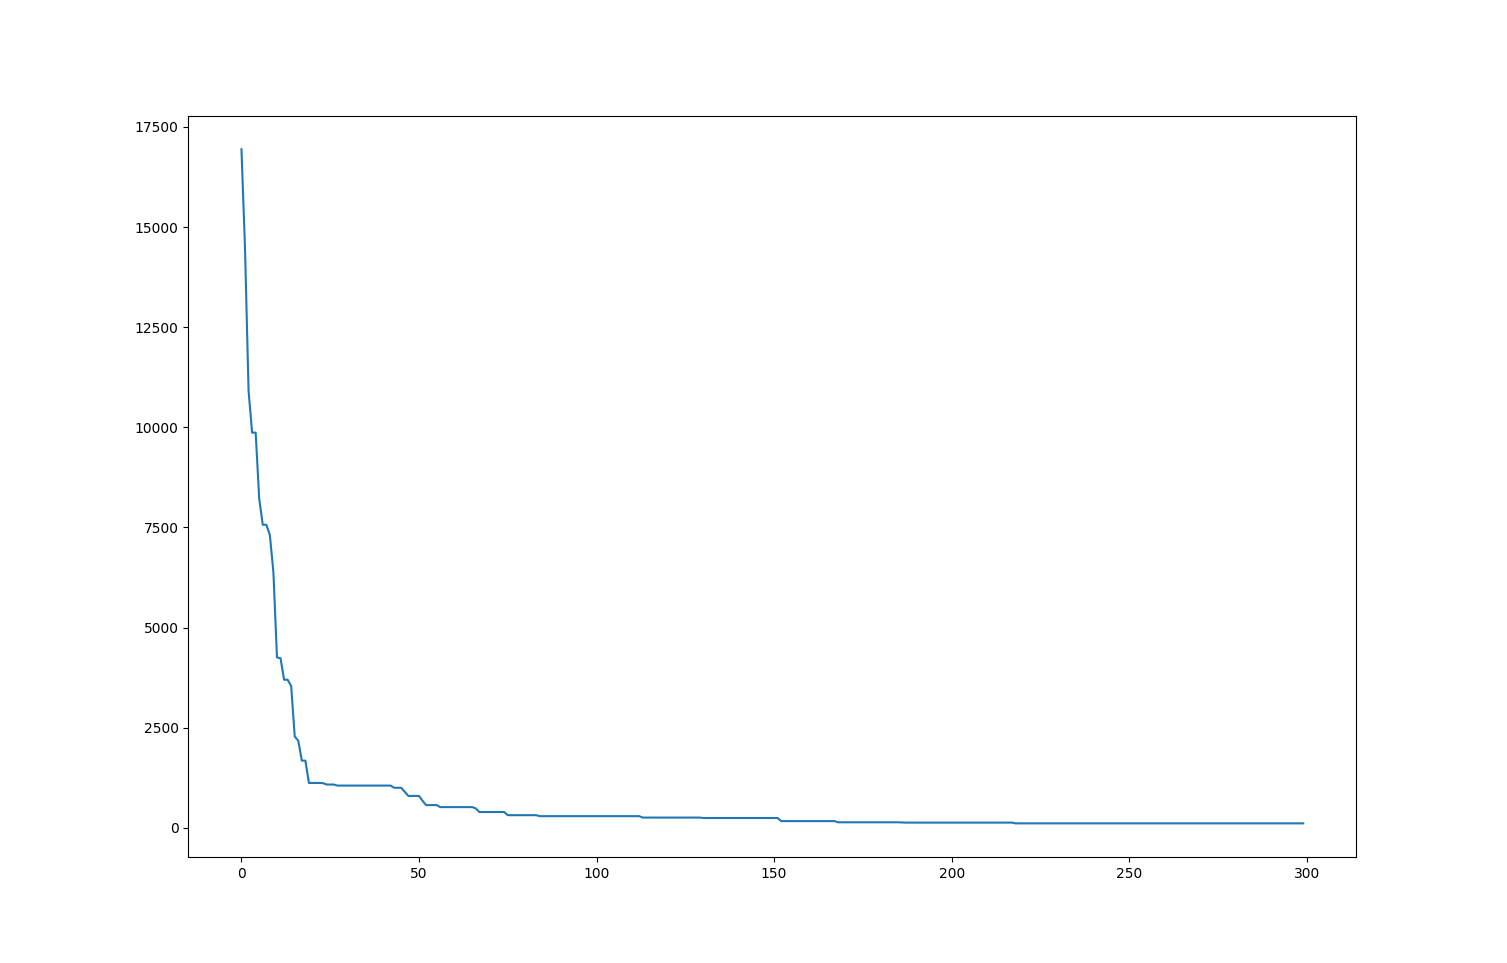
\includegraphics[scale=0.3]{plots/bb4.png}
    \end{center}
\end{frame}

\begin{frame}{Black-Box 5}
    \begin{center}
    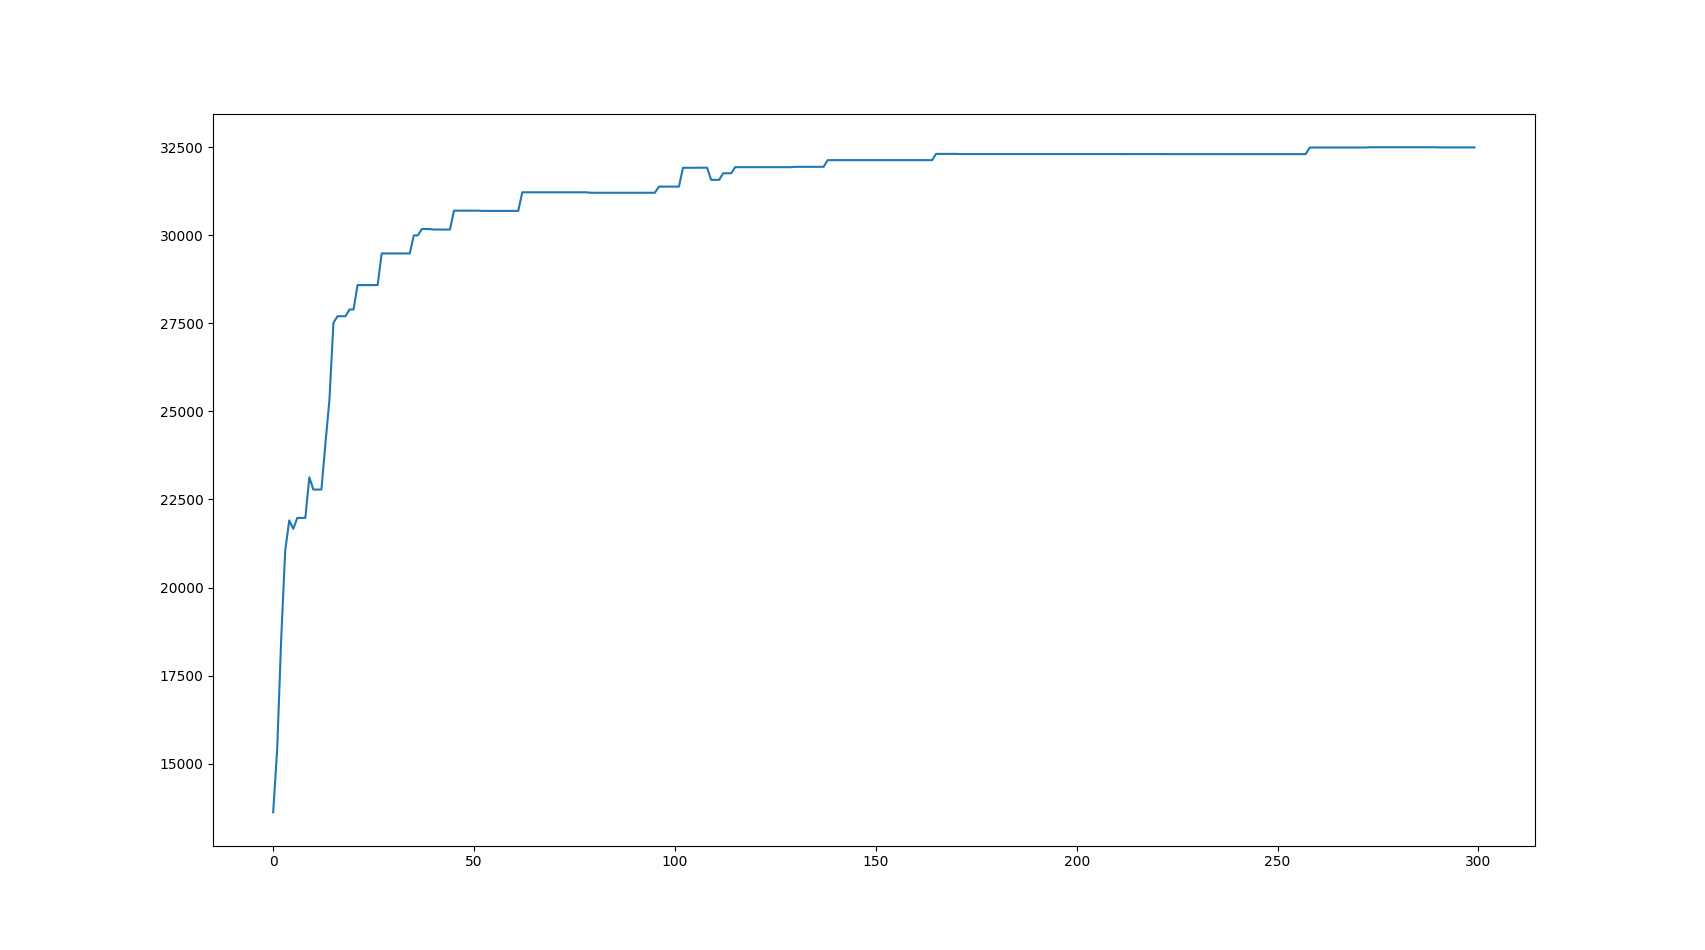
\includegraphics[scale=0.25]{plots/bb5.png}
    \end{center}
\end{frame}

\begin{frame}{Beste Blackbox für Verfahren?}
Lässt sich eine Aussage treffen, bei welcher Blackbox dieses Verfahren am besten funktioniert?
Können Sie sich denken, weshalb?
    \begin{itemize}
    \item BB1: schwankt stark $\Rightarrow$ funktioniert schlecht
    \item BB2: konvergiert schnell gegen kleine Werte $\Rightarrow$ funktioniert gut
    \item BB3: schwankt stark $\Rightarrow$ schlecht
    \item BB4: konvergiert gegen kleine Werte $\Rightarrow$ gut
    \item BB5: konvergiert gegen größere Werte $\Rightarrow$ gut
    \item $\Rightarrow$ BB2, BB5 & BB5 scheinen alle recht gut zu funktionieren.
    \end{itemize}
\end{frame}


\begin{frame}{Effizienter machen?}
Ist dieses Verfahren effizient? Wie könnte man das Verfahren leicht(!) abwandeln, um ein (noch)
effizienteres Verfahren zu erhalten?
    \begin{itemize}
    \item Sobald man merkt, dass die BB auf größer/kleiner werdende Werte anspringt Bereich der Zufallszahl anpassen. Man wählt dann also zwischen [current-best, MAXVALUE] oder [MINVALUE, current-best]. 
    \end{itemize}
\end{frame}

\end{document}
% Local Variables:
% TeX-engine: xetex
% End:
